\section{Performance Analysis}
\label{analysis}
% 对于Contention based的机制, RNTI保持多久??ca depend de la hypothese...(on peut consider la duree d'allocation)
% L'argument est 1) reduction de nb de messages echages 2)...
A comparative performance analysis between traditional RACH and our proposal (network integrated M2M-orientated polling service) is presented in this section. We focus on the consumption of RBs  (used for data transmission and signaling), the minimum number of RNTI, for both methods.

\subsection{System model}
\begin{figure}[!t]
	\centering
	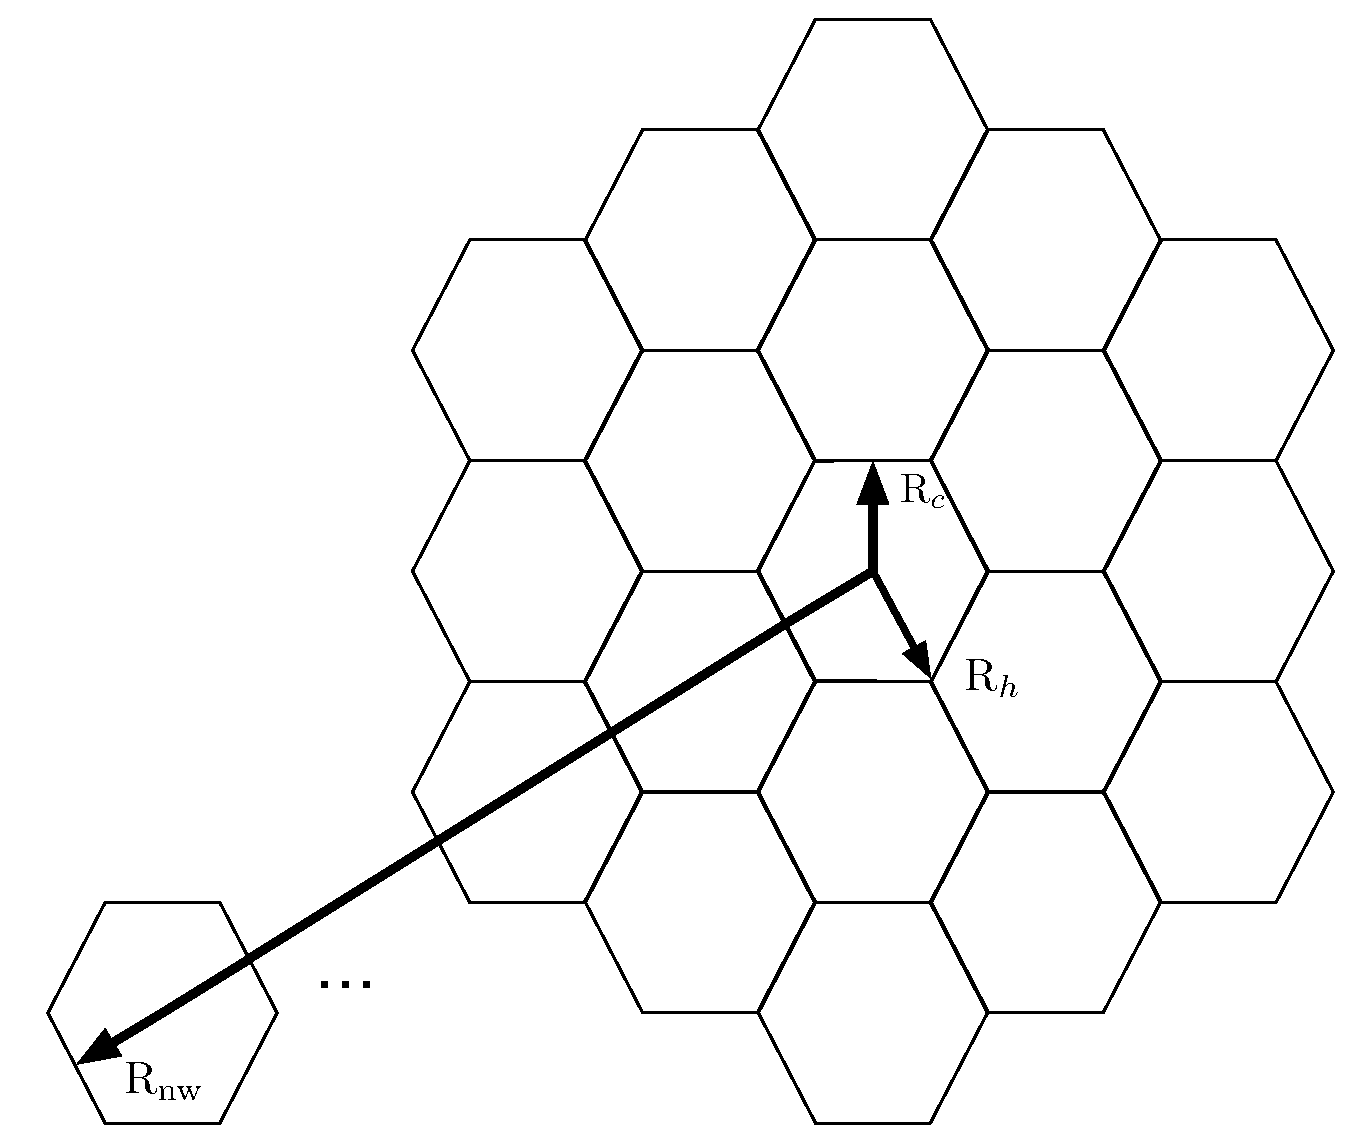
\includegraphics[width=0.9\linewidth]{Chapter6/Figures/hexagone_grid}
	\caption{The studied hexagonal grid network topology}
	\label{fig:hexagone_grid}
\end{figure}
We consider a regular hexagonal networks. Its topology is illustrated in Fig.~\ref{fig:hexagone_grid}, where $R_{\text{nw}}$ refers to the network coverage radius and $R_c$ denotes the half distance between two adjacent eNBs.
Performance analysis for a regular hexagonal grid network can be well approximated by the fluid model proposed in~\cite{kelif2010fluid} (shown in Fig.~\ref{fig:fluid_model}). The key idea of such a model consists in replacing a given fixed finite number of interfering sources (e.g. eNBs) by an equivalent continuum of transmitters. The latters are spatially uniformly distributed in the network.

The amount of MTC devices served by each eNB, denoted by $N_d$, is assumed to be very large, e.g, can reach up to $15000$. These devices are static and periodically sending data in uplink. The device reporting period $T$ is assumed to a random variable whose distribution is unknown. Due to the lack of statistics about reporting periods in the literature, we assume that the range of $T$ is assumed to be concentrated between $1$ min and $24$ hours. To avoid the possible collision, the report moment is chosen uniformly between time interval $\left[ 0, T\right] $. 

The volume of each transmission varies from $100$ bytes to $1000$ bytes.\qs{Is it necessary to consider the packet length follow pareto distribution?} Radio link conditions are ideal and data reporting is finished in the first transmission. 

BS have omnidirectional antenna so that a BS covers a single cell. For the downlink channel, all eNB transmit with the same power. Fading and shadowing are averaged out. The path loss function $g_{u,b}(r)= Kr^{-\eta}$, where $K$ is a constant, $r$ is the distance between $u$ and $b$ and $\gamma$ is the path-loss exponent. In the uplink, fractional power control is taken into account. The power compensation factor is denoted by $\alpha$
%	\item The system can be described as follows: first the device requests polling service, indicating the reporting period. Then the base station grants access and schedules the device to transmit in specific time intervals, allowing an efficient sharing of the resources among all the devices in the cell in a coordinated way. 
\subsection{System model}
\begin{figure}[!t]
	\centering
	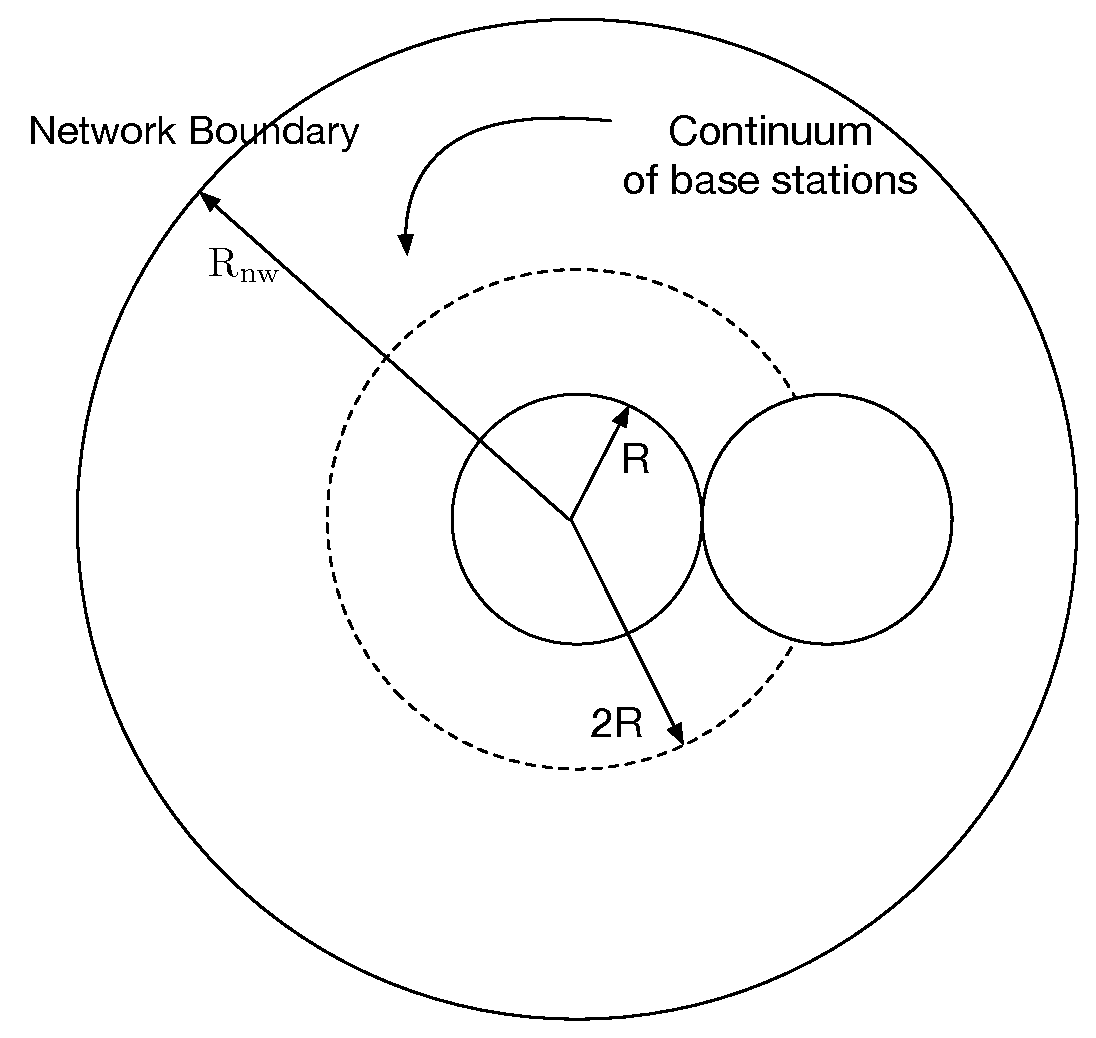
\includegraphics[width=0.9\linewidth]{Chapter6/Figures/fluid_model}
	\caption{Fluid model illustration}
	\label{fig:fluid_model}
\end{figure}


\subsection{Lower bound of RNTI required}
Let $C_{\text{min}}$ be the low bound of RNTI required in the coverage zone of an eNB.

\subsubsection{Our proposal}
In a system with our proposed multiple period polling service, the number of occupied RNTI (i.e. PRD-RNTI) depends on the amount of device $N_d$ served by the eNB and polling period. Recall that eNB provides $K$ available polling periods. The polling period is denoted by $T_{n}$, where $T_n = 2^n \cdot W \cdot T_f$. The number of devices with the same polling period is denoted by $g_{n}$. For polling period $T_n$, there exist $2^n$ available polling windows. Thus with $g_n$ device, it needs at least $\frac{g_n}{2^n}$ RNTI to satisfy all devices. Similarly, it should provide at least $C_{min}$ RNTI satisfying the following formula:  
\begin{align}	
 C_{\text{min}} = \sum_{n=0}^{K} \frac{g_n}{2^n} \label{eq:lower-bound}
\end{align}

\subsubsection{Random access method}
As discussed in previous section, once that RNTI is allocated, it will be occupied within time duration $T_{\text{in}}$, which is the expiration time of RRC inactivity timer. Let $C_{\text{RNTI}}$ be the total occupied RNTI number within $T_{\text{in}}$.

For conventional random access method, let's consider a certain periodic M2M application which deploys $N$ MTC devices having the same reporting period $T$. Within time duration $T_{\text{in}}$, the probability that one device occupies one RNTI (i.e. transmits a packet) is $T_{\text{in}}/T$. Since RRC inactivity timer is typically set as $10$ seconds~\cite{scjha2014} and random variable reporting period $T$ is mainly distributed between $1$ min and $24$ hours, thus, the probability $T_{\text{in}}/T$ is usually very small.

Actually, the $C_{\text{RNTI}}$ follows binomial distribution, however, when $N$ is big enough, $C_{\text{RNTI}}$ can be approximated regarded to follow poisson distribution. Similarly, the occupied RNTI by other periodic M2M applications also follows poisson distribution.
Since the reporting behavior among different periodic M2M applications deployed in a LTE system is independent, we can thus think the total occupied RNTI number follows poisson distribution.

How to calculate the average of $C_{\text{RNTI}}$ (i.e. the intensity of poisson distribution)?. 
We just need to consider the central eNB in Fig.~\ref{fig:fluid_model}. Recall that $N_{d}$ is the amount of M2M devices deployed in the coverage area of this eNB. Hence, the location of M2M devices form a Binomial Point Process (BPP). Given that $N_d$ is assumed to be enough big, the BPP can be well approximated by a Poisson Point Process $\Phi_m$ with spatial intensity $\lambda_m = N_d / \pi R^2$.

Consider a given M2M device with index $i$. Its reporting period is $T_i$. The probability $p$ that one RNTI is occupied by this device is $T_{\textbf{in}}/T_i$. The probability that the total occupied RNTI is zero can be expressed as follows:
\begin{align}
	\label{eq:void_proba_step_1}
	\mathbf{P} \left\lbrace  C_{\text{RNTI}} = 0 \right\rbrace  = \mathbb{E} \left[ \prod_{r_i \in \Phi_m}^{} 1 -  \frac{T_{\textbf{in}}}{T_i} \right] ,
\end{align}
where $r_i$ refers to distance between the considered device and eNB located at the origin, $T_i$ is a random variable whose distribution is unknown. The subscript $i$ can be omitted for the sake of readability. According to campbell theory, \eqref{eq:void_proba_step_1} can be further simplified: 
\qs{Acutally LPGL...} 
\begin{align}
	\label{eq:rnti_nb_void_proba}
	\mathbf{P} \left\lbrace  C_{\text{RNTI}} = 0  \right\rbrace  &= \mathbb{E}_{\Phi_m} \left[ \prod_{r \in \Phi_m}^{} \mathbb{E}_{T} \left[ 1 - \frac{T_{\text{in}}}{T} \right] \right] \nonumber\\
	&= \exp\left\lbrace -\mathbb{E}_{T} \left[ \int_{0}^{R} \frac{T_{\text{in}}}{T} 2\pi r \lambda_m dr  \right] \right\rbrace \nonumber\\
	&= \exp\left\lbrace -\lambda_m \pi R^2  T_{\text{in}} \mathbb{E}_{T} \left[ \frac{1}{T}  \right] \right\rbrace \nonumber \\
	&= \exp\left\lbrace -N_{d} T_{\text{in}}/\mathbb{E}_T \left[ \frac{1}{T} \right]\right\rbrace. 
\end{align}

From \eqref{eq:rnti_nb_void_proba}, we deduce that the average of $C_{\text{RNTI}}$ is:
\begin{align}
	\lambda &= N_{d} T_{\text{in}}/\mathbb{E} \left[ \frac{1}{T} \right],
\end{align}
% ===============================================
% Qipeng Song: The following section is the inital version used in VTC2015 paper. Now I think it is not correct.
%For a Poisson process, during a duration of RRC Inactivity timer $T_{in}$, the number RNTI occupied by devices $C_{RNTI}$ is a random variable respecting Poisson distribution with an intensity: 
%\begin{align}
%\lambda = N_{d}T_{in}/\mathbb{E}[T]
%\end{align}
%where $N_{d}$ is total number of MTC devices and $\mathbb{E}[T]$ is the expectation of reporting period To reduce random request collision, 
% ===============================================
Recall that $C_{\text{RNTI}}$  follows poisson distribution, the minimum number of RNTI required $C_{\text{min}}$ should satisfy the probability where $C_{\text{RNTI}}$ is less than $C_{min}$ is greater than a predefined threshold, for example $0.99$. Thus, the low bound of required RNTI $C_{\text{min}}$ can be calculated as follows:
\begin{align}	
\label{eq:low-bound-rach}
C_{\text{min}} &= \min \left\lbrace \mathbf{P} \{ C_{RNTI} < C_{min} \} \geq \text{Threshold} \right\rbrace \nonumber \\
&= \min \left\lbrace M: \sum_{n=0}^{M} \frac{\lambda ^ n }{ n! } e^{-\lambda} \geq \text{Threshold} \right\rbrace 
\end{align}






With OFDMA on the downlink or with SC-FDMA on the uplink, there is no (or limited if we consider inter-carrier interference) intra-cell interference. The single-carrier frequency-division multiple access method that is implemented in the uplink of LTE-Advanced introduces additional requirements to performs cheduling. That is, the PRBs that the SFDS algorithm allocates for a UE must be continuous in the frequency domain. Thus, it is reasonable to assume that channel suffers multiple path fading.


Our model, called the fluid model in [12], the central cell is modeled by a disk of radius Rc and is surrounded by several rings of interfering cells at distances $2nR_c (n =1, 2, ...)$. The network size can be expressed as $R_{nw} =(2N_c+1)R_c$, where $N_c$ represents the number of rings.



\subsection{Resource Blocks consumption}
%Compared with traditional random procedure requiring at least messages exchanged before data transmission, our proposed service allows device directly sending data packet thus reduce the Resource Block consumption. In random access procedure, RACH preamble in step 1 consists of $XX$ bytes. RAR in step 2 consists of a temporary C-RNTI which holds $4$ bytes.Contention resultion identity in step 3/4 is usually made from S-TMSI and has $6$ bytes. In total, 
%For a small payload less than $100$ bytes, 
%% http://blog.sina.com.cn/s/blog_927cff010101926v.html
%RA preamble generally requires $6$ Resource Blocks.
%% http://wireless.itri.org.tw/MPFiles/M2-1409-LTE_MAC_Intro_PartII.pdf
%Overhead in RAR is $4$ bytes.
%Resolution contention identity in L2/L3 messages is It $5$ octets.
%Contention solution echo $5$ octets.
% Please add the following required packages to your document preamble:
% \usepackage{booktabs}
Comparing Fig.~\ref{fig:lte-ra} and Fig.~\ref{fig:Comparison}, we observe that in the uplink direction data transmission with conventional random access should at least first send four signaling messages: random access preamble, RRC ConnectionRequest, RRC ConnectionSetupComplete and RRC ConnectionReconfigurationComplete while it requires zero message with our proposal. For the downlink direction, our proposal economizes the resources used for RAR, RRC ConnectionSetup, RRC ConnectionReconfiguration and RRC Connection release messages. That mens that our proposal can effectively reduce signaling overhead for small payload and energy consumption. 
 
The MTC devices have previously attached to network and transmit a $100$-byte payload. Random access collision is not taken into account. 

\begin{table}[h]
	\centering
	\caption{RRC messages exchanged between UE and the eNB (unit: bit)}
	\label{tab:economized-bytes}
	\resizebox{0.9\textwidth}{!}{%
		\begin{tabular}{@{}lcccccc@{}}
			\toprule
			RRC Message Name                  & \thead{Payload \\Size} & \thead{MAC \\ Header} & \thead{RLC \\ Header} & \thead{PDCP \\Header} & Downlink & Uplink \\ \midrule
			ConnectionSetupRequest            & 48           & 72         & 8          & 8           &          & 136    \\
			ConnectionSetup                   & 320          & 72         & 8          & 8           & 408      &        \\
			ConnnectionSetupComplete          & 56           & 16         & 8          & 8           &          & 88     \\
			ConnectionReconfiguration         & 632          & 16         & 8          & 8           & 664      &        \\
			ConnectionReconfigurationComplete & 16           & 16         & 8          & 8           &          & 48     \\
			ConnectionRelease                 & 16           & 16         & 8          & 8           & 48       &        \\ \midrule
			Economized Bytes Number           & \multicolumn{4}{l}{}                                 & 1120     & 272    \\ \bottomrule
		\end{tabular}%
	}
\end{table}

To get the exact RRC message payload size, we do a realistic measurement with \qs{Here we should add figures...} capture the exchange traffic between a UE and eNB. The economized bytes number, in uplink and downlink, are resumed in Table.~\ref{tab:economized-bytes}. The bytes related to security and integrity are ignored. The PDCP protocol header occupies $1$ bytes, RLC header occupies $1$ bytes. The header of MAC layer is a little complicated. Normaly MAC header takes $2$ bytes, however, before contention resolution stage, the MAC layer should contain a random number as temporary UE identifier ($6$ bytes) and an associated subheader ($1$ bytes).
%Besides reduction of required RNTI, we proposed service also could reduce the number of needed signaling messages. Due to the limit of time, we will develop a model to estimate performance gain in terms of signaling overhead.


\subsubsection{Downlink Signaling Resource Block Consumption}
We take the signaling message RRC ConnectionReconfiguration as example, to estimate how many RBs are consumed within one TTI for the downlink channel in a hexagonal cell (the coverage area of the central eNB shown in Fig.~\ref{fig:hexagone_grid}). This message contains $664$ bits (i.e. $83$ bytes, resumed in Tab.~\ref{tab:economized-bytes}).

Taken from~\cite[Tab.~7.1.7.2.1-1]{lte-eutra-physical-layer}, the transport block size (TBS) of bits that can be carried by a single RB in LTE with different modulation coding scheme (indicated by TBS index) is resumed in the left two columns in Tab.~\ref{tab:tbs-distance}. Since the TBS should be transmitted within one TTI, $10$ ms in LTE, there exists one minimum SNR requirement for each modulation coding schema. 

Normally, this SNR threshold can be calculated via inversing the widely used Shannon channel capacity formula. However, the latter in practice cannot accurately describe the channel capacity due to the ignorance of several implementation issues. Hence, we use one modified Shannon formula adjusted by simulation results proposed in~\cite{mogensen2007lte}. This formula is as follows:
\begin{align}
	\label{eq:debit_with_respect_sinr}
	S &= \beta B \eta  \log_2 \left( 1 + \frac{\Theta}{\Theta_{\text{ref}}} \right) , \\
	\label{eq:sinr_threshold}
	\Theta &= \Theta_{\text{ref}} \left(  2^{\frac{S}{\beta B \eta  }} - 1 \right) ,
\end{align}
where $S$ (with unit of bits per second) is the date rate, $\alpha$ adjusts for the system bandwidth (BW) efficiency of LTE , $\Theta_{\text{ref}}$ adjusts for the SNR implementation efficiency of LTE.  Using curve fitting to the obtained simulation results, $\beta$ is set as $0.83$ and $\Theta_{\text{ref}}$ is set as $1.25$ (namely $1$dB)~\cite{mogensen2007lte}.  Parameter $B$ refers to the spectrum bandwidth occupied for transmission and is set as $180$ KHz in the case of one RB, $\Theta$ is the received SNR. The factor $\eta$ is a correction factor which nominally should be equal to one. Applying \eqref{eq:sinr_threshold}, the minimum SNR threshold to guarantee a certain data rate  can be calculated.

Given that one packet transmission is affected by path attenuation (fading and shadowing are assumed to be averaged out), we know the received SNR varies with respect to the distance to the cell center $r$. Due to scheduling algorithm and OFDMA multiplexing, the eNB during a given TTI only transmits to a certain device. Thus, there is no intra-cell interference. The interfering sources are other transmitting eNB. Under such assumption, reference~\cite{kelif2010fluid} gives the function between SNR $\Theta$ and distance to the disk cell center $r$:
\begin{align}
	\label{eq:sinr_with_repsect_distance}
	\Theta &= \frac{\gamma - 2}{4\pi\sqrt{3}/3} 
	\frac{(1 -\frac{r}{2R_c})^{\gamma - 2}}{(\frac{r}{2R_c})^{\gamma}}, \nonumber\\
	&= \frac{\gamma - 2}{4\pi\sqrt{3}/3} 
	\frac{(1 -\frac{\nu}{2})^{\gamma - 2}}{(\frac{\nu}{2})^{\gamma}},
\end{align}
where $R_c$ is the intersite distance, $\gamma$ is the path-loss exponent, $\nu$ is the relative distance (to the cell radius) in the cell, 


The area of a cell is $1/\rho_{\text{BS}} = \pi R^2$ with $R = R_c \sqrt{2\sqrt{3}/\pi}$.So, we integrate $f_u$ on a disk of radius $R$.
Combining \eqref{eq:sinr_threshold} and \eqref{eq:sinr_with_repsect_distance}, we observe that if one device needs to satisfy the SNR threshold, there exists a maximum distance to the cell center for $r$. Thus, the coverage area of the central eNB can be divided into a series of $M$ rings in which the device can use the same amount of RBs.
Let $N_{\text{RB}}(\text{MSG}, i)$ the RB consumption for one device in ring $i$. Given that the probability that one device is located in the ring with index $i$ is:
\begin{align}
	p(i) 
	&= \nu_{\text{u,i}}^{2} - \nu_{\text{l,i}}^{2},
\end{align}
where $\nu_{\text{u,i}}$ and $\nu_{\text{l,i}}$ are respectively the upper and low bound of ring $i$.
Thus, the average RB consumption within one TTI, for downlink signaling message is expressed as follows:
\begin{align}
	\overline{N_{\text{RB}}} = \sum_{i=0}^{M} N_{\text{RB}}(i) p(i)
\end{align}




\begin{align}
	D &= \sqrt{3} r_{H}, \\
	r_{eq} &= \sqrt{\frac{\sqrt{3}}{2\pi}} D
\end{align}


We assume that the device always use the highest MCS if possible. To calculate the average RB consumption during one TTI in a cell, we can do a simple integration over the disk area. Thus, 

%\begin{align}
%	p(i) = \nu_{\text{upper}}^{2} - \nu_{\text{low}}^{2}
%\end{align}


\begin{align}
	\overline{N_{\text{RB}}}  &= \frac{1}{\pi R} 2 \pi \int_{r_{\text{low, i}}}^{r_{\text{upper, i}}} N_{\text{RB}}(\text{MSG})  dr \\
	&=  \frac{1}{ \sqrt{\frac{\sqrt{3}}{2\pi}} D }2 \int_{r_{\text{low, i}}}^{r_{\text{upper, i}}} N_{\text{RB}}(\text{MSG})  dr \\
	&=  \frac{2}{ \sqrt{\frac{\sqrt{3}}{2\pi}} } N_{\text{RB}}(\text{MSG})  \int_{r_{\text{low, i}}}^{r_{\text{upper, i}}} d (\frac{r}{D}) \\
	&=  \sum_{i=0}^{M}   N_{\text{RB}}(\text{MSG})[(\frac{r_{\text{upper}, i}}{D})^2 - (\frac{r_{\text{lower}, i}}{D})^2] ,
\end{align}
\begin{align}
	\overline{N_{\text{RB}}}  &= \frac{1}{\pi R^2}2 \pi \int_{r_{\text{low, i}}}^{r_{\text{upper, i}}} N_{\text{RB}}(\text{MSG})  dr \\
	&=  \frac{1}{ \sqrt{\frac{\sqrt{3}}{2\pi}} D }2 \int_{r_{\text{low, i}}}^{r_{\text{upper, i}}} N_{\text{RB}}(\text{MSG})  dr \\
	&=  \frac{2}{ \sqrt{\frac{\sqrt{3}}{2\pi}} } N_{\text{RB}}(\text{MSG})  \int_{r_{\text{low, i}}}^{r_{\text{upper, i}}} d (\frac{r}{D}) \\
	&=  \sum_{i=0}^{M}   N_{\text{RB}}(\text{MSG})[(\frac{r_{\text{upper}, i}}{D})^2 - (\frac{r_{\text{lower}, i}}{D})^2] ,
\end{align}
where $M$ is the number of rings divided by RB numbers.
%\begin{align}
%	N \sum_{i=0}^{M}\frac{r_{i+1}^2 - r_{i}^{2}}{r_{eq}^2} N_{\text{RB}}
%\end{align} 
\subsubsection{Uplink data transmission Resource Block Consumption}
Similar methodology can be applied to estimate the RB consumption for data transmission in the uplink. The significant difference is about the function between SNR and distance between device and eNB. In reference~\cite{coupechoux2011set}, uplink performance in LTE network are analyzed under fluid model. Fractional power control is taken into account. 
$\rho_{m}$, the scheduled devices intensity at a given
Relative location $\nu = \frac{r}{2R}$ $R = $
Given by~\cite[Eq.(10)]{coupechoux2011set} The SINR expression in uplink is as follows:
\begin{align}
	\Theta_{\text{uplink}} = \frac{r^{-\eta(1 - \alpha)}}{ 8 \sum_{n=1}^{\infty} n^{\alpha \eta +2 - \eta} I_{n}\left( \alpha, \eta\right) },
\end{align}
\begin{align}
	\Theta_{\text{uplink}} = \frac{r^{-\eta(1 - \alpha)}}{ 2 \pi \rho_{m} \sum_{n=1}^{\infty} (2nR)^{\alpha \eta +2 - \eta} I_{n}\left( \alpha, \eta\right) },
\end{align}
where $I_{n}\left( \alpha, \eta\right) = \int_{0}^{\frac{1}{2n}} x^{\alpha \eta} \left[ (1-x)^{1-\eta} +  (1 +x)^{1 - \eta} \right] dx$. Term $I_{n}\left( \alpha, \eta\right)$ refers to the contribution of the $n^{\text{th}}$ ring to the external interference.

The total interference $I_{\text{ext}}$ caused by other eNB than the central one is composed by $N_c$ component, namely $I_{\text{ext}} = \sum_{n=1}^{N_c} I_{\text{n, ext}}$.


We can still rely on \eqref to evaluate the RB consumption.
\subsection{Numeric result}
From the above analysis, the lower bound of RNTI required both in our proposal and random access procedure depends the distribution of reporting period $T$. Even though lots of MTC applications have been proposed in recently years, the deployment of MTC on a large scale is still an expectation. Hence, there is no well-established distribution about reporting period. Performance analysis is conducted in two cases: $T$ respects log-normal distribution and uniform distribution. Similar analysis can be made for other distributions. 
\subsubsection{Log-normal distribution}
We suppose that logarithm of  user-defined reporting period $T$ (unit of hour), namely $\ln T$,  is a random variable respecting normal distribution $N (\mu, \sigma^2)$. The mean of $\ln T$ is $0$. The probability of T in interval $1$ min and $24$ hours is great than $68.27 \%$ and less than $95\%$. Thus, 
% ln(24) = 3.18 
% ln(1.0/60) = -4.09
% ln(2.0/60) = -3.40
% u-sigma_max <= -4.09 ==> sigma_max >= 4.09 => we could take 4.2
% u-2*sigma_min <= -4.09 ==> sigma_min >= 2.04  => we could take 2.1
we take $0$ for $\mu$ and $\sigma$ should be in range $\lbrack1.6, 3.2\rbrack$. To reduce complexity of problem, we make some approximation when estimating the mean of $T$: regarding all reporting periods less than $1$ min as $1$ min and all periods great than $24$ hours as $24$ hours. 
%Therefore, the mean of reporting period $T$ is represented as shown in formula (\ref{eq:T-expectation}).
%\begin{align}
%	f_{T}(x) &= \frac{1}{\sigma \sqrt{2\pi}x} \exp -\frac{(\ln x )^2}{2\sigma^2} \nonumber \\
%	E[T] &=\frac{1}{60}P\{ T= 1 min\} + \int_{\frac{1}{60}}^{24} t \cdot f_{T}(t) dt +24P\{ T= 24 hour\} \nonumber \\
%	& = \frac{1}{60}\Phi (\frac{\ln 1/60}{\sigma}) +  \Phi (\frac{\ln 24}{\sigma}) -\Phi (\frac{\ln 1/60}{\sigma}) + 24 \cdot ( 1-\Phi (\frac{\ln 24     }{\sigma}))
%	\label{eq:T-expectation} 	
%\end{align}
Supposing number of LTE frame in a single polling window $W$ is set as $10$. To cover the range from $1$ min to $24$ hours. The minimum supported polling period in our proposal is set as $51.2$ sec and the maximum supported polling period as $104857.6$ sec , almost $29.13$ hours. According to Eq.\ref{eq:period-conversion}, the supported polling period list is $51.2$ sec, $102.4$ sec, $204.8$ sec, $409.6$ sec, ..., $52428.8$ sec, $104857.6$ sec. Polling period $T_n$ is thus a discrete random variable.
% whose probability distribution is the following: 
%\begin{align}
%	& P\{ T_n = N \} = \Phi(\frac{\ln 2N}{\sigma}) - \Phi(\frac{\ln N}{\sigma}) , n=1,2...N_{max}-1 \nonumber \\
%	%						   	\shortintertext{For the minimum and maximum supported polling period:}
%	& P\{ T_0 = N \} = \Phi(\frac{\ln N}{\sigma}) \nonumber \\
%	& P\{ T_{N_{max}} = N \} = 1- \Phi(\frac{\ln N-0}{\sigma}) \nonumber 					   
%\end{align}
Given distribution of each polling period and total MTC device in system model, the consumption of PRD-RNTI in RACH and periodic polling case could be estimated by formula \ref{eq:lower-bound} and \ref{eq:low-bound-rach}. Two cases where $\mu=0, \sigma=1.6$ and $\mu=0, \sigma=3.2$ are shown in Fig.\ref{fig:log-normal-RNTI-consumption}.
\begin{figure}[!t]
	\centering
	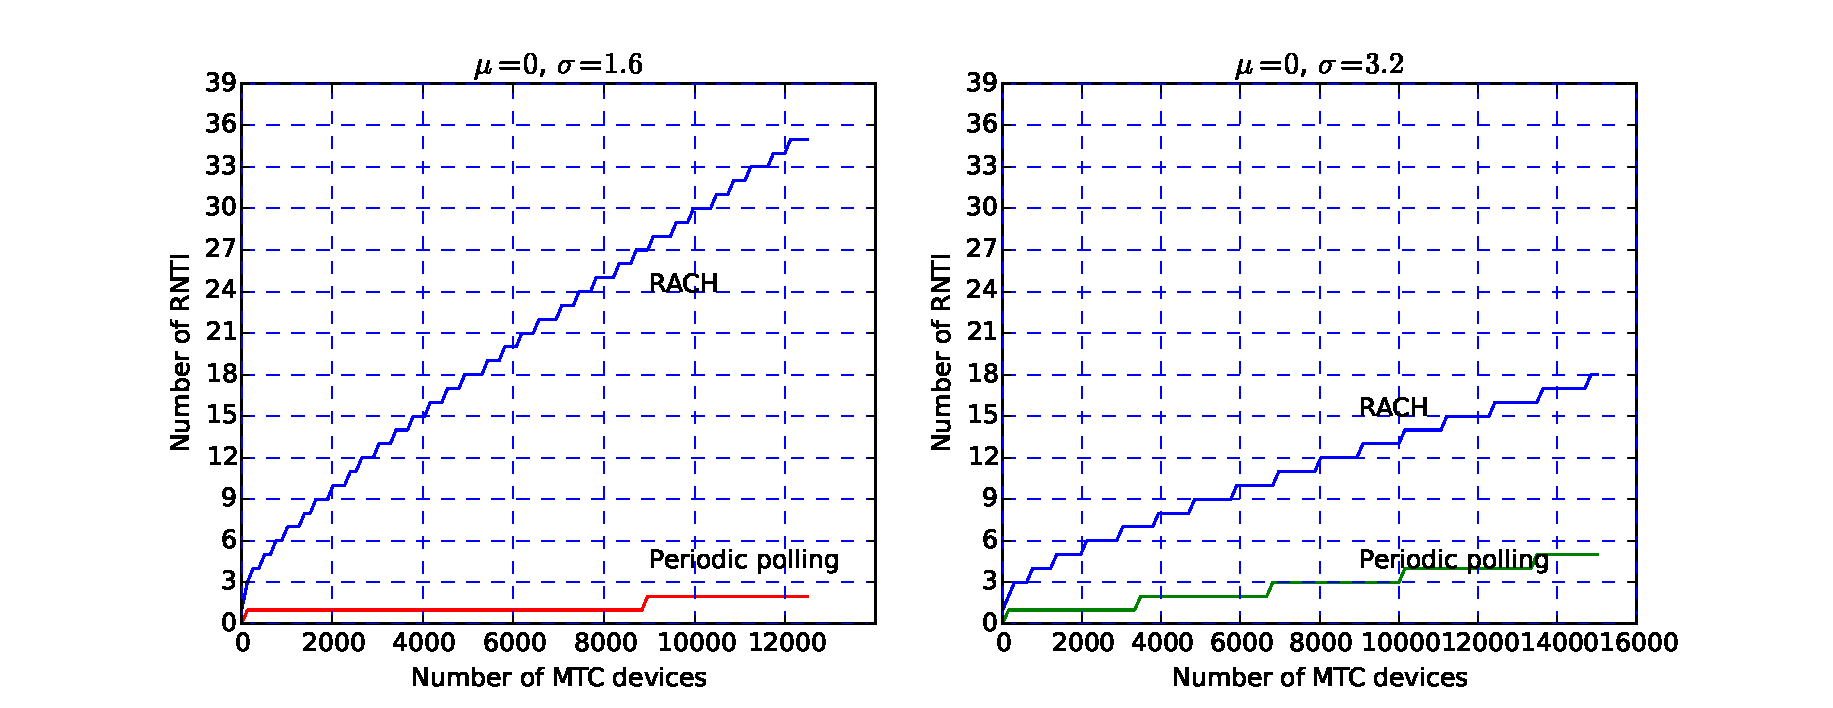
\includegraphics[width=\linewidth]{Chapter6/Figures/log-normal.eps}
	\caption{Comparison of RNTI required for case of log-normal distribution}
	\label{fig:log-normal-RNTI-consumption}
\end{figure}

\subsubsection{Uniform distribution}
We suppose in this case user-defined reporting period $T$ respects uniform distribution between $1$ min and $24$ hours. Obviously the mean of $T$ is equal to $12$ hours. Given total device number and the repartition of each polling period 
%$$
%f_T(x) = \left\{ \begin{array}{rl}
%0.04170 &\mbox{ if $x \in \lbrack 0.01666, 24\rbrack$} \\
%0 &\mbox{ otherwise}
%\end{array} \right.
%$$
it is not difficult to get the probability distribution for each eNB supported polling period and estimate device repartition, and further estimate the minimum required RNTI for both case according to formula (\ref{eq:lower-bound}) and (\ref{eq:low-bound-rach}). The comparison result is shown in Fig.\ref{fig:uniform-RNTI-consumption}.

\begin{figure}[!t]
	\centering
	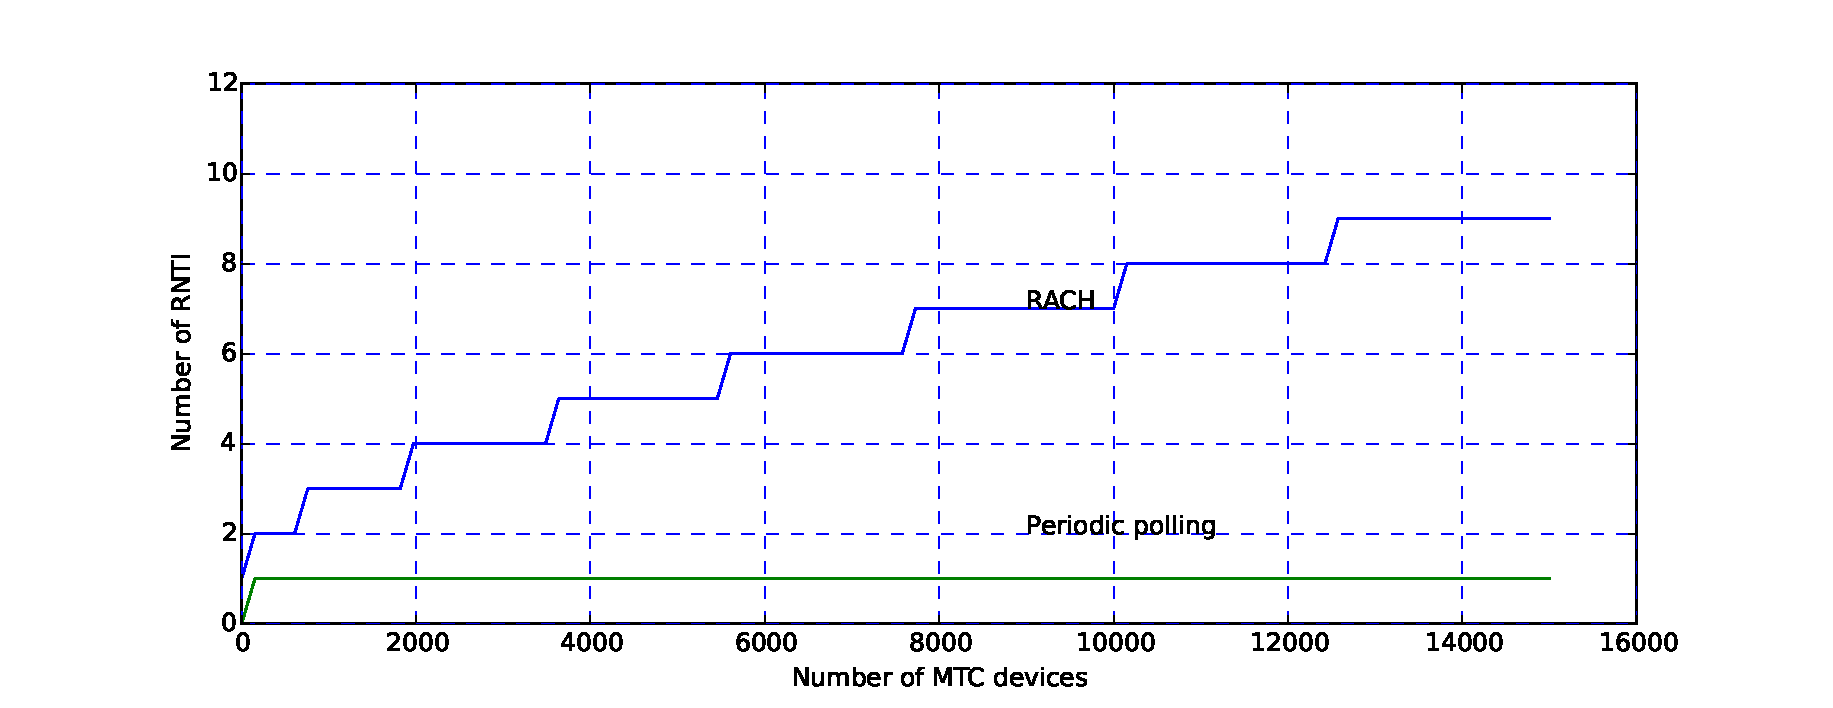
\includegraphics[width=\linewidth]{Chapter6/Figures/uniform.eps}
	\caption{Comparison of RNTI required for case of uniform distribution}
	\label{fig:uniform-RNTI-consumption}
\end{figure}

\subsubsection{Pareto distribution}
We suppose that user-defined reporting period $T$ follows pareto distribution that always greater than $1$ min. The cumulative distribution function of Pareto distribution is:
\begin{align}
	F_T(t) = 1 - (\frac{T_{\text{min}}}{t})^{\alpha}, t \geq T_{\text{min}} 
\end{align}
where $\alpha$ is the shape parameter. To make sure that most values of $T$ are within $\left[1 min, 24 hours \right] $, let $T_{\text{min}}  = 60 $seconds, $\alpha = 1$. Now we can estimate $\mathbb{E}[T] = 120$ seconds. 

\subsubsection{RB consumption}
we can calculate the maximum relative location that allows to use the given MCS. The results are shown in the forth column in Tab.~\ref{tab:tbs-distance}. The RB number required to transmit $664$ bits, under each MCS, are listed in the rightmost column of Tab.~\ref{tab:tbs-distance}. For example, for MCS represented by TBS index $26$, just one RB is sufficient to transmit $664$ bits, while for TBS index $1$, up to $19$ RB are needed.


According to Tab.~\ref{tab:tbs_sinr_dist} and given that $r/D$ value interval is $\left[ 0, 0.58\right] $. the cell can be divided into a series of ring in which the eNB consume the same RB to transmit RRC signaling to devices. The limiter distance series $\left[0,  0.25\right] $, $\left[0.25,  0.38\right] $, $\left[0.38,  0.43\right] $, $\left[0.43,  0.46\right] $, $\left[0.46,  0.49\right] $, $\left[0.49,  0.52\right] $, $\left[0.52,  0.56\right] $, $\left[0,.56  0.5859\right] $.
\begin{table}
	\centering
	\begin{tabular}{rrllr}
		\toprule
		TBS Index &  TBS & SINR Threshold & Max Dist. &  RB Nb \\
		\midrule
		0 &   16 &           0.10 &     0.706 &     42 \\
		1 &   28 &           0.17 &     0.657 &     24 \\
		2 &   36 &           0.23 &     0.634 &     19 \\
		3 &   52 &           0.34 &     0.600 &     13 \\
		4 &   60 &           0.40 &     0.586 &     12 \\
		5 &   72 &           0.50 &     0.568 &     10 \\
		6 &   88 &           0.63 &     0.547 &      8 \\
		7 &  112 &           0.85 &     0.522 &      6 \\
		8 &  128 &           1.01 &     0.507 &      6 \\
		9 &  148 &           1.23 &     0.491 &      5 \\
		10 &  164 &           1.43 &     0.479 &      5 \\
		11 &  188 &           1.74 &     0.463 &      4 \\
		12 &  220 &           2.22 &     0.443 &      4 \\
		13 &  244 &           2.63 &     0.430 &      3 \\
		14 &  276 &           3.25 &     0.413 &      3 \\
		15 &  300 &           3.78 &     0.402 &      3 \\
		16 &  316 &           4.17 &     0.395 &      3 \\
		17 &  348 &           5.03 &     0.381 &      2 \\
		18 &  388 &           6.31 &     0.364 &      2 \\
		19 &  420 &           7.52 &     0.352 &      2 \\
		20 &  452 &           8.93 &     0.340 &      2 \\
		21 &  500 &          11.47 &     0.324 &      2 \\
		22 &  532 &          13.50 &     0.313 &      2 \\
		23 &  564 &          15.86 &     0.303 &      2 \\
		24 &  596 &          18.60 &     0.293 &      2 \\
		25 &  628 &          21.78 &     0.284 &      2 \\
		26 &  740 &          37.47 &     0.253 &      1 \\
		\bottomrule
	\end{tabular}
	\caption{TBS, SNR threshold and distance table}
	\label{tab:tbs-distance}
\end{table}


\begin{tabular}{rllrr}
	\toprule
	RB Nb & Lower Bound & Max Dist. &  TBS Index &  SINR Threshold \\
	\midrule
	1 &       0.000 &     0.253 &         26 &       37.471797 \\
	2 &       0.253 &     0.381 &         17 &        5.032093 \\
	3 &       0.381 &     0.430 &         13 &        2.627502 \\
	4 &       0.430 &     0.463 &         11 &        1.740310 \\
	5 &       0.463 &     0.491 &          9 &        1.233814 \\
	6 &       0.491 &     0.522 &          7 &        0.851753 \\
	8 &       0.522 &     0.547 &          6 &        0.630284 \\
	10 &       0.547 &     0.568 &          5 &        0.495761 \\
	12 &       0.568 &     0.586 &          4 &        0.401222 \\
	\bottomrule
\end{tabular}





Similar methodology can be used to estimate the RB consumption for other signaling messages. Finally, we find that at least ... RB are required for 


For the uplink, the compensation factor $\alpha$ is set as $0.1$ (refer to Fig.~$3$ in~\cite{coupechoux2011set}).
%\begin{table}[!t]
%	\renewcommand{\arraystretch}{1.3}
%	\caption{Comparison}
%	\label{tab:message-exchanged-comparison}
%	\centering
%	\begin{tabular}{lcc}
%		\hline
%		item & random access  & multiple period polling service\\
%		\hline
%		number of sent signaling messages & 4 & 0\\
%		\hline
%		number of transmitted bytes & $ \approx $ 100 & 0 \\
%		\hline
%		number of resource bloc & 6 & 14 \\
%		\hline
%	\end{tabular}
%\end{table}

Some remarks from our numerical results :
\begin{inparaenum}[\itshape a\upshape)]
	\item  Our proposal can effectively mitigate the random access congestion caused by massive MTC devices in radio access network, since a considerable partition of MTC traffic exhibits periodicity and can avoid random access procedure using our proposed multiple period polling service.
	\item  with our proposal, in both log-normal and uniform case, a single cell supports up to fifteen thousand devices with less than five RNTI, which has a better performance than conventional random access procedure and largely exceeds the expectation of many optimists.
	\item If $T$ respects uniform distribution, then it just needs one RNTI to support up to $15000$ devices, which gains enormous optimization compared with the case of random access.
	\item In case that reporting period $T$ respects log-normal distribution, the lower bound of RNTI required depends mean and variation of $T$. The more concentrated the reporting period, the less RNTI required.
\end{inparaenum} 